\documentclass[spanish]{udpreport}
\usepackage[utf8]{inputenc}
\usepackage[spanish]{babel}
\usepackage[]{float}

\title{Informe Nº2 Redes De Datos}

\author{Javiera Araya,
       Benjamin Morales,
        Fabian Estefania,
        Nicolas Pino.\\
        Profesor:Jaime Álvarez.\\
        Ayudante:Maximiliano Vega.} 

\begin{document}
\maketitle

\tableofcontents
\chapter{Resumen  }

El reciente laboratorio se tuvo como objetivos poder crear paquetes para luego enviarlos por red y que otros equipos pudieran recibir dicho paquete, para poder lograr dicho propósito se hace uso de dos programas, el primero es un programa interactivo llamado Scapy el cual permite crear además de otras muchas funciones que cumple. Por otro lado el segundo programa utilizado fue Wireshark el cual proporciona la captura de los paquetes enviados por Scapy.
Se realizaron múltiples envíos de paquetes trabajando sobre la capa 2, es decir a nivel de direccionamiento físico (MAC) probando distintas modalidades para observar que sucedía, con ello se obtuvo una visión general de cómo funcionaba el envió de estos paquetes cuando en emisor determina como enviar el paquete a través de la red en la cual estaba ubicado considerando fundamentalmente el tipo de topología en el cual se encuentra dicho emisor.



\chapter{Introducción }
 
En el presente informe se hace referencia a la importancia de crear paquetes y enviarlos a través de la red, el cual permitirá testear el funcionamiento que tiene este tipo de acciones dependiendo de cómo se trazan las rutas de envió. 
La característica fundamental de  tener el conocimiento de cómo crear y manipular paquetes ya que se tiene la visión de cómo es la trama o estructura del paquete que enviaremos,   para ello se determinan partes de dicha trama como la sincronización entre el emisor y receptor el cual se tiene que determinar en el inicio de la creación del paquete. Indistintamente, hay otras partes de la trama que se son de importancia como el tipo de dato que se introducirá en la creación del paquete, este puede ser un dato especifico, vacío como también invalido, esto dependerá de lo que quiera realizar el emisor del mensaje y el efecto que quiera realizar al enviar su paquete a uno o más destinatarios.
Otro aspecto a considerar es por qué capa se envía el paquete, es decir, se puede enviar mediante la capa 2 el cual trabaja sobre el direccionamiento físico (MAC), aunque también se puede enviar a través de la capa 3 la cual trabaja a nivel de red  el modelo TCP/IP, donde se manejan protocolos tales como ARP, IP, ICMP. Como enviemos este paquete dependerá de quien será adjudicado como el destinatario de nuestro envió. 




\chapter{Desarrollo}

\section{Creacion de paquetes}
\large Como primer paso a seguir se inicio la herramienta de creacion de paquetes llamada "Scapy", para iniciar esta aplicacion se procedio a ejecutar el comando "sudo scapy" 
para iniciarla, una vez hecho esto se continuo creando las distintas capas de un paquete (capa de enlace,red,transporte) y finalmente el payload.\\

Para crear una capa de enlace se debe crear una variable y asignarle los valores del comando Ether() (ejemplo: Enlace = Ether() ). Se pueden ver todos los campos de la variable creada con el comando "ls(variable)"\\
\begin{figure}[H]
\begin{center}
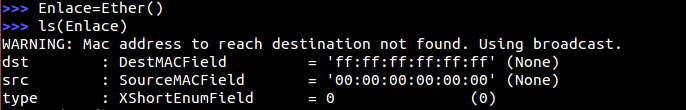
\includegraphics[scale=0.7]{images/1.png}
\end{center}
\end{figure}

Una vez desplegada la informacion de la variable podemos observar que tiene dos campos con direcciones MAC, el campo "dst" es la direccion MAC a la que se enviara el paquete, y el campo "src" es la direccion MAC de origen.\\

Se puede modificar los campos de la variable usando el comado con el nombre de la variable previamente asignado seguido de un punto y el nombre del campo que se desea modificar (ejemplo: Enlace.dst="ff:ff:ff:ff:ff:ff")\\

\begin{figure}[H]
\begin{center}
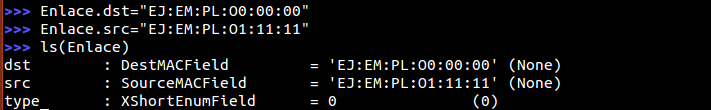
\includegraphics[scale=0.7]{images/6.png}
\end{center}
\end{figure}

\vspace{14cm}

El siguiente paso es crear la capa de red del paquete, para esto se debe crear una variable y asignarle los valores del comando IP() (ejemplo: Red = IP() ). Se pueden ver todos los campos de la variable creada con el comando "ls(variable)"\\

\begin{figure}[H]
\begin{center}
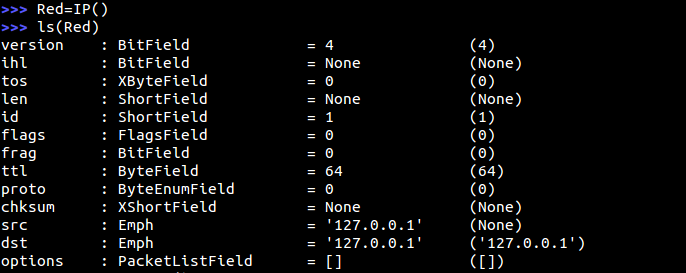
\includegraphics[scale=0.7]{images/2.png}
\end{center}
\end{figure}

Luego se debe crear la capa de transporte, se debe crear una variable y asignarle los valores del comando  ICMP() (ejemplo: Transporte = ICMP() ). Se pueden ver todos los campos de la variable creada con el comando "ls(variable)"\\

\begin{figure}[H]
\begin{center}
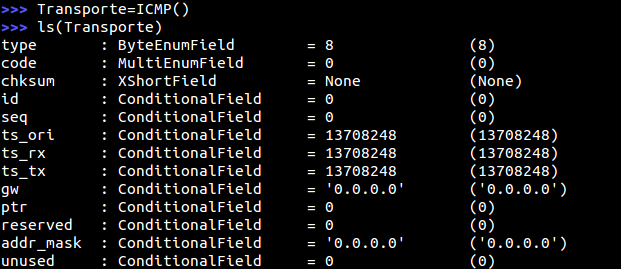
\includegraphics[scale=0.7]{images/3.png}
\end{center}
\end{figure}

\vspace{14cm}

Para finalizar la creación de variables se debe crear una y asignarle el contenido de el comando Raw() (ejemplo: Payload = Raw() ). Se pueden ver todos los campos de la variable creada con el comando "ls(variable)"\\

\begin{figure}[H]
\begin{center}
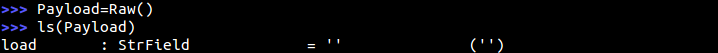
\includegraphics[scale=0.7]{images/4.png}
\end{center}
\end{figure}

Una vez creadas y asignadas todas las variables es momento de formar el paquete apilando todas las varibles por orden de capas según la pila OSI.\\
(ejemplo: paquete=Enlace/Red/Transporte/Payload)

\begin{figure}[H]
\begin{center}
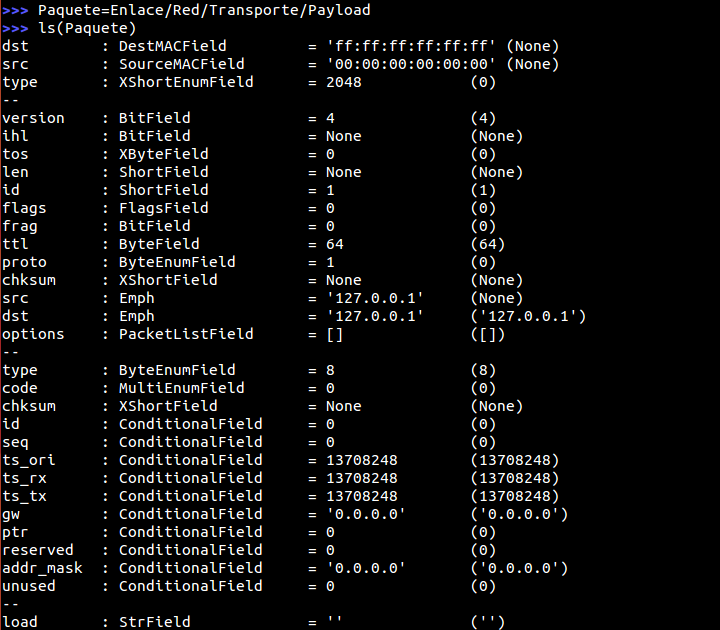
\includegraphics[scale=0.7]{images/5.png}
\end{center}
\end{figure}


\section{Envio de paquetes a travez de switch}
\subsection{Envio de paquete broadcast}

Para enviar paquetes de tipo broadcast a travez de la red se debe cambiar la direccion MAC de destino en la variable en la que tenemos asignada la capa de enlace, para esto se debe el proceso explicado en el punto 3.1 y asignar la MAC  de tipo broadcast (ff:ff:ff:ff:ff:ff)\\
\begin{figure}[H]
\begin{center}
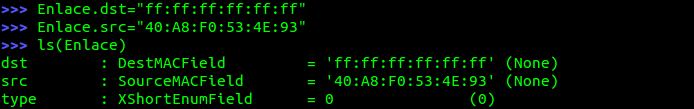
\includegraphics[scale=0.7]{images/switch1.png}
\end{center}
\end{figure}
Una vez cambiada la direccion MAC de destino, se debe volver a apilar el paquete y luego proceder a enviarlo con el comando sendp(Paquete).\\
\begin{figure}[H]
\begin{center}
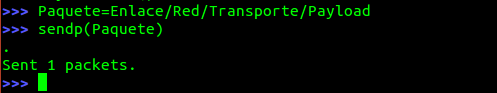
\includegraphics[scale=0.7]{images/switch2.png}
\end{center}
\end{figure}

Una vez enviado, el paquete llego a todos los equipos conectados al switch.

\subsection{Envio de paquete a MAC existente en la red}

Para enviar paquetes con una MAC de destino especifica a travez de la red se debe cambiar la direccion de destino en la variable en la que tenemos asignada la capa de enlace, para esto se debe el proceso explicado en el punto 3.1 y asignar la MAC del equipo que se desee que llegue el paquete.\\
\begin{figure}[H]
\begin{center}
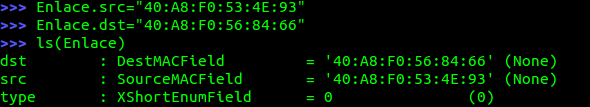
\includegraphics[scale=0.7]{images/switch3.png}
\end{center}
\end{figure}
\vspace{14cm}
Una vez cambiada la direccion MAC de destino, se debe volver a apilar el paquete y luego proceder a enviarlo con el comando sendp(Paquete).\\
\begin{figure}[H]
\begin{center}
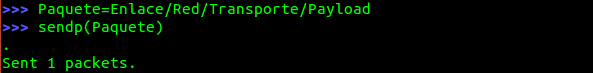
\includegraphics[scale=0.7]{images/switch4.png}
\end{center}
\end{figure}
Una vez enviado, el paquete solo llega al equipo que tiene la MAC especificada previamente en la capa de red.

\subsection{Envio de paquete a MAC inexistente en la red}

En este caso se sigue el mismo proceso que en los casos anteriores solo que esta vez utlizamos una MAC de destino que no existe dentro de la red. luego de enviar el paquete a travez de la red aparece un mensaje el cual da una advertencia de que la MAC de destino no existe dentro de la red y que se usara broadcast para enviar el paquete, por lo que este llego a todos los equipos de la red.
\begin{figure}[H]
\begin{center}
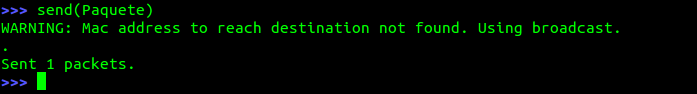
\includegraphics[scale=0.7]{images/switch5.png}
\end{center}
\end{figure}

\vspace{14cm}
\section{Envio de paquetes a travez de Hub}

\subsection{Envio de paquete broadcast}
Para enviar paquetes de tipo broadcast a través de la red se debe enviar el paquete a través del comando sendp(Paquete).  \\

Una vez enviado, el paquete llego a todos los equipos conectados al Hub
\begin{figure}[H]
\begin{center}
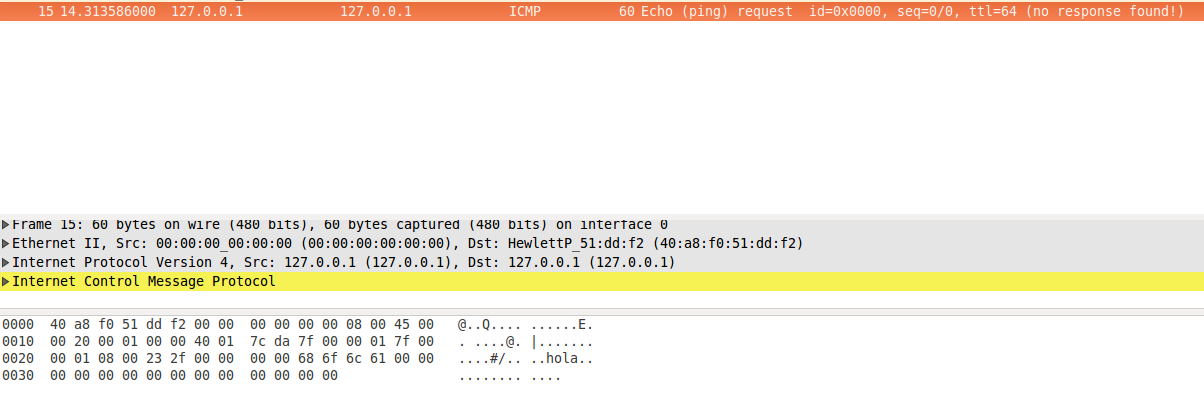
\includegraphics[scale=0.4]{images/Hub1.png}
\end{center}
\end{figure}
(equipo cualquiera conectado al Hub reciviendo el paquete enviado)
\vspace{14cm}
\subsection{Envio de paquete a MAC existente en la red}
Es imposible enviar un paquete a una MAC de destino específico de la red a través del hub, debido a que al momento de proceder a enviar el paquete con el comando sendp(paquete), al recibir el paquete el hub, este reenvía a todos los equipos conectados el paquete enviado.
\begin{figure}[H]
\begin{center}
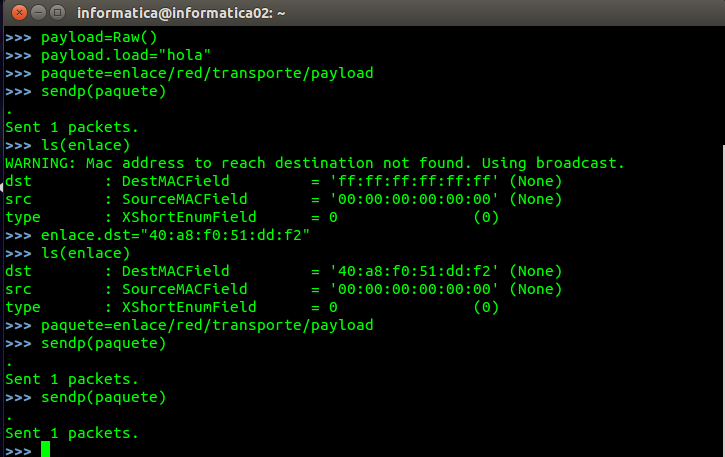
\includegraphics[scale=0.7]{images/Hub2.png}
\end{center}
\end{figure}
(enlace lleva una dirección MAC de un PC conectado al Hub como destino)
\vspace{14cm}
\subsection{Envio de paquete a MAC inexistente en la red}
Al momento de enviar el paquete con una MAC no perteneciente a la red, aparece un mensaje el cual da una advertencia de que la MAC de destino no existe dentro de la red y que se usara broadcast para enviar el paquete, por lo que este llego a todos los equipos de la red.
\begin{figure}[H]
\begin{center}
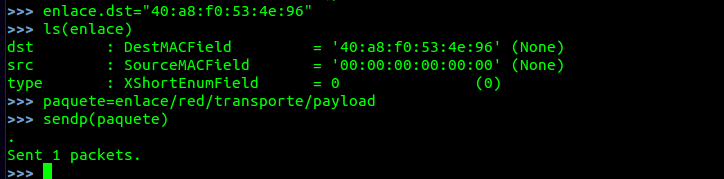
\includegraphics[scale=0.7]{images/Hub3.png}
(enlace lleva una dirección MAC de un PC desconectado del Hub)
\end{center}
\end{figure}




\vspace{12cm}
\chapter{Cuestionario}
\section{¿Qué pasa cuando envió un paquete a la dirección\\ FF:FF:FF:FF:FF:FF? ¿Quienes
lo reciben? ¿Por qué?}

La direccion FF:FF:FF:FF:FF:FF es la direccion por defecto del broadcast, esto significa que el destino del paquete son todos los equipos conectados a la red, por lo que el paquete es recepcionado por todos los equipos conectados, esto pasa tanto en el switch como en el hub.

\section{¿Qué pasa cuando envió un paquete a una MAC de otro\\ equipo? ¿Quieres lo pueden reciben? ¿Por qué?}

En caso de que estemos utilizando un switch, el paquete sera recibido  unicamente por el equipo que posea la direccion MAC especificada en el destino del paquete, esto sucede ya que el switch es capaz de identificar las direcciones de cada equipo y redireccionar el paquete a un equipo especifico.\\

Por otro lado el Hub no tiene la capacidad de identificar las direcciones y lo que hace es enviarlo a todos los equipos conectados al Hub, todos los equipos reciben el paquete y deciden si dececharlo o no.

\section{¿Qué sucede si envía un paquete a una MAC que no\\ corresponda a ningún equipo de la red? ¿Quienes lo\\ pueden recepcionar? ¿Por qué?}
El equipo detecta automaticamente que tal MAC no existe dentro de la la red, por lo tanto utiliza el sistema broadcast para enviar el paquete a todos los equipos conectados al switch o Hub.
\chapter{Conclusión}

Del presente informe se concluyen los siguientes aspectos sobre la creación de paquetes y el posterior envió de ellos a través de la red. Primero se discutieron los aspectos sobre el envió de estos a través de equipos conectados a un switch realizándose tres tipos de envió el primero fue enviarlo a un equipo con su MAC especifica el cual no hubo problemas con la llegada del paquete a la MAC de destino, posteriormente se envía el mismo paquete a todos los equipos conectados a la red teniendo una acogida favorable y finalmente, dentro de esta misma actividad realizamos el envió de el mismo paquete a una MAC de destino no existente en la red, como resultado se obtuvo  fue relevante debido a que el computador del cual se operaba mando una advertencia señalando que dicha MAC de destino no existía y que por ende enviaría el paquete como destinatario Broadcast el cual llego favorablemente a todos los equipos.

 De esta primera actividad realizada hay puntos importantes los cuales se destacaran el primero y fundamental fue que el envío de paquetes se desarrolló usando al final de la trama o frame un relleno para el paquete en vez de haberlo enviado con una confirmación de recepción por parte del usuario (CRC), de haber enviado esto con CRC a cada equipo el cual recibió el paquete enviado debió de haber confirmado, esto hubiese servido de noción para el que emitió dicho mensaje tuviera la certeza de que lo que envío llego bien a su destino. 
Otro aspecto muy importante a considerar y obviamente destacar fue que al realizar envíos a todos los computadores conectados a la red  y a un destino que no se encuentre en la red, en ambos casos llego a todos los computadores de la red, esto es extraño debido a que   al estar conectado en un Switch este filtra todos los frames según las direcciones MAC, al enviarlo por broadcast se estaría enviando paquetes un numero incontable de veces lo cual no seria el mejor de los casos considerando que el Switch filtra los paquetes que enviamos, esto pudo deberse a la naturaleza del Switch con el que trabajamos o también por algún tipo de configuración realzada a dicho equipo.

Lo segundo que se discute para profundizar más sobre el funcionamiento de envíos de paquetes se hace en relación a las mismas tres actividades realizadas solo que la conexión es a través de un Hub el cual se trabajó con tres computadores y se fue checkeando su funcionamiento en cada acción de envío que se realizó y en todos los casos al mandar un paquete ya fuera por MAC específica, Broadcast o enviando a una MAC fuera de la red de conexión a dicho Hub, este paquete llegaba igualmente a todos los computadores conectados a dicho equipo. De lo anterior se puede deducir que ocurre por la función que realiza un Hub en otras palabras al ser un concentrador, centraliza todas las redes conectadas, para luego al enviar un paquete este lo amplia por toda la red conectada llegando a todos los computadores que están en el Hub. 
Con lo que se realizó en ambas actividades se tuvo una mayor comprensión de cómo se mueve  un envío a través de la red intentando diversos métodos el cual ampliaban enormemente la visión de las rutas que puede tomar el remitir un paquete.



\end{document}